%! Author = Omar Iskandarani
%! Title =  Beyond Spacetime: A Fluid-Dynamic Theory of Gravity and Time from Vorticity
%! Date = 6/20/2025
%! Affiliation = Independent Researcher, Groningen, The Netherlands
%! License = © 2025 Omar Iskandarani. All rights reserved. This manuscript is made available for academic reading and citation only. No republication, redistribution, or derivative works are permitted without explicit written permission from the author. Contact: info@omariskandarani.com
%! ORCID = 0009-0006-1686-3961
%! DOI = 10.5281/zenodo.15706547
\newcommand{\paperdoi}{10.5281/zenodo.15706547}


\documentclass[a4paper,12pt]{article}
\usepackage{../vamstyle}
\usepackage{subfiles}
\usepackage{subcaption}
\usepackage{tikz}
\usepackage{amsmath}
\usepackage{amssymb}
\usepackage{hyperref}
\usetikzlibrary{arrows.meta, positioning, shapes.multipart}
\usetikzlibrary{shapes.geometric, arrows.meta, positioning}
\tikzstyle{block} = [rectangle, draw, rounded corners, text centered, minimum height=2em, text width=4.5cm, fill=blue!5]
\tikzstyle{arrow} = [thick, ->, >=Stealth]
\usepackage{pgfplots}
\pgfplotsset{compat=1.17}
\usetikzlibrary{arrows.meta, decorations.pathmorphing}
\usepackage{amsthm}
\usepackage{booktabs}
\usepackage{array}
\usepackage{bm}



\title{
    \textbf{Beyond Spacetime: A Fluid-Dynamic Theory of Gravity and Time from Vorticity}\\[0.5em]
    \large A Mathematical Formulation of Temporal and Topological Dynamics in an Incompressible Æther Medium\\[0.5em]
}
\author{
    Omar Iskandarani\thanks{
        Independent Researcher, Groningen, The Netherlands.\\
        Email: \texttt{info@omariskandarani.com}\\
        ORCID: \href{https://orcid.org/0009-0006-1686-3961}{0009-0006-1686-3961}\\
        DOI: \href{https://doi.org/10.5281/zenodo.15706547}{10.5281/zenodo.15706547}
    }
}
\date{\today}


\begin{document}
    \maketitle
    \vspace{-2ex}


    \begin{abstract}
        This document presents a mathematical treatment of vorticity and time structure within the framework of the Vortex Æther Model (VAM), a fluid-dynamic reformulation of gravitation and temporal evolution. It introduces the core vorticity equation in natural coordinates, derived from the dynamics of an incompressible, inviscid æther medium. By interpreting vorticity as a measure of atomic clock delay, we couple swirl energy to experienced time and obtain expressions for vorticity in terms of local velocity gradients and flow curvature.

        The appendices develop key substructures of VAM, including the topological and energetic conditions that trigger irreversible events, called \textbf{Kairos moments}, where the flow evolution becomes non-analytic. These singularities partition æther-time into epochs and correspond to phenomena such as vortex reconnection, swirl pressure rupture, or helicity discontinuities. Each temporal mode—\textbf{Aithēr-Time} (\( \mathcal{N} \)), \textbf{Chronos-Time} (\( \tau \)), \textbf{Swirl Clock} (\( S(t) \)), and \textbf{Vortex Proper Time} (\( T_v \))—is formally defined and related to physical vortex observables.

        Altogether, this work formulates a temporally stratified æther theory with experimentally testable dynamics, replacing spacetime curvature with a framework in which time dilation and mass-energy interactions emerge from structured vorticity fields.

        The derivations build upon the classical foundations laid by Helmholtz's theory of vortex invariants~\cite{helmholtz1858integralsvortex}, Maxwell's fluid-based model of electromagnetic stress~\cite{maxwell1861pressure}, and subsequent developments in shear-layer vorticity and planetary flow dynamics~\cite{lamb1932, rossby1939}.


    \end{abstract}


    \vfill
%
    \newpage
    \tableofcontents
    \newpage


    \appendix
    \def\standalonechapter{false}
        \section{Fundamentals of Æther Fluid Motion and Vorticity}

    \subsection{Fundamental Assumptions}
    The Æther is modeled as a homogeneous, incompressible, and inviscid fluid. This implies constant density:
    \begin{equation}
        \frac{d \rho}{d t} = 0.
    \end{equation}

    We adopt a Cartesian coordinate system \((x, y, z)\) fixed in absolute space. The velocity field \(\vec{u} = (u, v, w)\) represents the local Æther flow:
    \begin{equation}
        u = \frac{dx}{dt}, \quad v = \frac{dy}{dt}, \quad w = \frac{dz}{dt}.
    \end{equation}

    Let \(P\) denote pressure, and \((X, Y, Z)\) the external force per unit volume acting in each direction.

    \subsection{Stress Equilibrium in Free Æther}
    The general stress equilibrium equations are:
    \begin{align}
        X &= \frac{\partial P_{xx}}{\partial x} + \frac{\partial P_{xy}}{\partial y} + \frac{\partial P_{xz}}{\partial z}, \\
        Y &= \frac{\partial P_{yx}}{\partial x} + \frac{\partial P_{yy}}{\partial y} + \frac{\partial P_{yz}}{\partial z}, \\
        Z &= \frac{\partial P_{zx}}{\partial x} + \frac{\partial P_{zy}}{\partial y} + \frac{\partial P_{zz}}{\partial z}.
    \end{align}

    Assuming irrotational flow, all shear stresses vanish:
    \begin{equation}
        P_{xy} = P_{xz} = P_{yz} = 0.
    \end{equation}

    Hence the simplified stress force equations become:
    \begin{equation}
        X = \frac{\partial P_{xx}}{\partial x}, \quad
        Y = \frac{\partial P_{yy}}{\partial y}, \quad
        Z = \frac{\partial P_{zz}}{\partial z}.
    \end{equation}

    The total force differential satisfies:
    \begin{equation}
        X\, dx + Y\, dy + Z\, dz = dV,
    \end{equation}
    where \(V\) is a scalar potential.

    Normal stresses are related to flow and pressure:
    \begin{align}
        P_{xx} &= \rho u^2 - P, \\
        P_{yy} &= \rho v^2 - P, \\
        P_{zz} &= \rho w^2 - P.
    \end{align}

    Substituting into the momentum equation yields:
    \begin{align}
        X &= \frac{D u}{D t} + \frac{1}{\rho} \frac{\partial P}{\partial x}, \\
        Y &= \frac{D v}{D t} + \frac{1}{\rho} \frac{\partial P}{\partial y}, \\
        Z &= \frac{D w}{D t} + \frac{1}{\rho} \frac{\partial P}{\partial z},
    \end{align}
    where the material derivative is:
    \begin{equation}
        \frac{D}{D t} = \frac{\partial}{\partial t} + \vec{u} \cdot \nabla.
    \end{equation}

    \subsection{Continuity Equation}
    For an incompressible fluid:
    \begin{equation}
        \nabla \cdot \vec{u} = \frac{\partial u}{\partial x} + \frac{\partial v}{\partial y} + \frac{\partial w}{\partial z} = 0.
    \end{equation}

    \subsection*{Velocity Potential and Irrotational Flow}
    If the flow is irrotational, a scalar potential \(\varphi\) exists such that:
    \begin{equation}
        \vec{u} = \nabla \varphi.
    \end{equation}
    This leads to the Laplace equation:
    \begin{equation}
        \nabla^2 \varphi = 0.
    \end{equation}

    \subsection{Vorticity and Circulation}
    In irrotational flow, the vorticity vector vanishes:
    \begin{equation}
        \vec{\omega} = \nabla \times \vec{u} = 0.
    \end{equation}

    In rotational flow, the components become:
    \begin{align}
        \omega_x &= \frac{\partial w}{\partial y} - \frac{\partial v}{\partial z}, \\
        \omega_y &= \frac{\partial u}{\partial z} - \frac{\partial w}{\partial x}, \\
        \omega_z &= \frac{\partial v}{\partial x} - \frac{\partial u}{\partial y}.
    \end{align}

    The circulation \(\Gamma\) over an infinitesimal closed loop is:
    \begin{equation}
        \Gamma = \oint \vec{u} \cdot d\vec{l} = \iint (\nabla \times \vec{u}) \cdot \hat{n} \, dA.
    \end{equation}

    \subsection{Energy of a Vortex}
    The kinetic energy of a rotating vortex region is:
    \begin{equation}
        E = \frac{1}{2} \rho \iiint |\vec{u}|^2 \, dV.
    \end{equation}

    Assuming solid-body rotation and edge tangential velocity \(c\), the vorticity magnitude is:
    \begin{equation}
        |\vec{\omega}| = \frac{c}{r}.
    \end{equation}

    Then the vortex energy simplifies to:
    \begin{equation}
        E = \frac{1}{2} M c^2,
    \end{equation}
    where \(M\) is the effective mass of the rotating Æther parcel.

    \subsection*{Conclusion}
    This appendix establishes the fluid-dynamic foundations of Æther theory under assumptions of incompressibility and inviscidity. It introduces the vorticity vector, velocity potential, and circulation as key constructs, which serve as a basis for gravitational analogs, time dilation, and vortex dynamics in the broader VAM framework.

  % Sets standalone=false
        \section{Vortex Pressure, Stress, and Vorticity}


    \subsection{Vortex Pressure Relations}
    In a steadily rotating vortex tube, let the core pressure be \(P_0\). The pressure at the vortex edge \(P_1\) is:
    \begin{equation}
        P_1 = P_0 + \frac{1}{2} \rho c^2,
    \end{equation}
    where \(\rho\) is the Æther density and \(c\) the tangential velocity at the vortex edge.

    The axial pressure parallel to the vortex tube is:
    \begin{equation}
        P_2 = P_0 + \frac{1}{4} \rho c^2.
    \end{equation}

    The transverse pressure difference becomes:
    \begin{equation}
        P_1 - P_2 = \frac{1}{4} \rho c^2.
    \end{equation}

    For irrotational vortices where pressure arises from distributed angular momentum (e.g. as in swirl clocks or quantized vortices), this generalizes to:
    \begin{equation}
        P_1 - P_2 = N \rho c^2,
    \end{equation}
    with \(N\) a coefficient dependent on angular profile and vortex density.

    \subsection{Stress Tensor Components}
    Define vortex orientation via direction cosines \(l, m, n\) with respect to the \((x, y, z)\) axes.

    The full stress tensor becomes:
    \begin{align}
        P_{xx} &= \rho c^2 l^2 - P_1, & P_{xy} &= \rho c^2 l m, & P_{xz} &= \rho c^2 l n, \\
        P_{yy} &= \rho c^2 m^2 - P_1, & P_{yz} &= \rho c^2 m n, & P_{yx} &= P_{xy}, \\
        P_{zz} &= \rho c^2 n^2 - P_1, & P_{zx} &= \rho c^2 n l, & P_{zy} &= P_{yz}.
    \end{align}

    If velocity components are defined by:
    \begin{equation}
        u = c l, \quad v = c m, \quad w = c n,
    \end{equation}
    then the stress tensor rewrites as:
    \begin{align}
        P_{xx} &= \rho u^2 - P_1, & P_{xy} &= \rho u v, & P_{xz} &= \rho u w, \\
        P_{yy} &= \rho v^2 - P_1, & P_{yz} &= \rho v w, & P_{yx} &= \rho v u, \\
        P_{zz} &= \rho w^2 - P_1, & P_{zx} &= \rho w u, & P_{zy} &= \rho w v.
    \end{align}

    \subsection{Equilibrium of Stresses and Force Components}
    The force per unit volume follows the momentum balance:
    \begin{align}
        X &= \frac{\partial P_{xx}}{\partial x} + \frac{\partial P_{xy}}{\partial y} + \frac{\partial P_{xz}}{\partial z}, \\
        Y &= \frac{\partial P_{yx}}{\partial x} + \frac{\partial P_{yy}}{\partial y} + \frac{\partial P_{yz}}{\partial z}, \\
        Z &= \frac{\partial P_{zx}}{\partial x} + \frac{\partial P_{zy}}{\partial y} + \frac{\partial P_{zz}}{\partial z}.
    \end{align}

    Using the velocity substitution, the identity:
    \[
        u \frac{\partial u}{\partial x} + v \frac{\partial v}{\partial x} + w \frac{\partial w}{\partial x} = \frac{1}{2} \frac{\partial}{\partial x}(u^2 + v^2 + w^2)
    \]
    leads to:
    \begin{align}
        X &= \frac{1}{2} \rho \frac{\partial}{\partial x}(c^2)
        + u \rho (\nabla \cdot \vec{u})
        - \rho v (2 \zeta) + \rho w (2 \eta)
        - \frac{\partial P_1}{\partial x}, \\
        Y &= \frac{1}{2} \rho \frac{\partial}{\partial y}(c^2)
        + v \rho (\nabla \cdot \vec{u})
        - \rho w (2 \xi) + \rho u (2 \zeta)
        - \frac{\partial P_1}{\partial y}, \\
        Z &= \frac{1}{2} \rho \frac{\partial}{\partial z}(c^2)
        + w \rho (\nabla \cdot \vec{u})
        - \rho u (2 \eta) + \rho v (2 \xi)
        - \frac{\partial P_1}{\partial z}.
    \end{align}

    \subsection{Connection to Vorticity and Coriolis Acceleration}
    The terms involving:
    \begin{equation}
        \frac{1}{2} \rho \frac{\partial}{\partial x} (u^2 + v^2 + w^2)
    \end{equation}
    can be interpreted as a \textbf{Coulomb-like acceleration} from local kinetic energy gradients.

    The cross terms:
    \begin{equation}
        - v (2 \zeta) + w (2 \eta),
    \end{equation}
    represent \textbf{Coriolis-type accelerations} in the rotating æther due to vorticity components in the transverse plane.

    \subsection*{Conclusion}
    This derivation exposes the deeper link between internal vortex pressure gradients and inertial forces resulting from vorticity. The decomposition of stresses into axial and transverse components reveals how Coriolis accelerations and pressure anisotropies arise naturally in rotating æther systems. These structures provide the mechanical foundation for VAM’s time dilation, mass generation, and vortex-induced gravitational fields.

    \begin{tcolorbox}[colback=gray!10, colframe=black, title=Example: Vortex Pressure Drop]

        Assuming:
        \[
            \rho = 7 \times 10^{-7} \, \mathrm{kg/m^3}, \quad c = \mathbf{v}_{\scriptscriptstyle\boldsymbol{\circlearrowleft}} = 1.09384563 \times 10^6 \, \mathrm{m/s}
        \]

        We compute:
        \[
            P_1 - P_0 = \frac{1}{2} \rho c^2 = \boxed{418{,}774.39 \, \mathrm{Pa}}, \qquad
            P_1 - P_2 = \frac{1}{4} \rho c^2 = \boxed{209{,}387.20 \, \mathrm{Pa}}
        \]

        This anisotropic pressure difference supports the vortex stability and creates a radial pressure gradient consistent with centripetal balance.
    \end{tcolorbox}

  % Sets standalone=false
        \section{Vorticity in Natural Coordinates}

    We define \( d\omega \) as the experienced time rate for atoms moving along natural coordinates in a vorticity field. Let us consider a central æther particle located at the core of a vortex, having no velocity potential. It satisfies:

    \begin{equation}
        \frac{\partial w}{\partial y} - \frac{\partial v}{\partial z} = 2\xi, \quad
        \frac{\partial u}{\partial z} - \frac{\partial w}{\partial x} = 2\eta, \quad
        \frac{\partial v}{\partial x} - \frac{\partial u}{\partial y} = 2\zeta.
    \end{equation}

    Since the æther particle remains fixed at the center, its local rotation is only about the \(Z\)-axis, leading to:

    \begin{equation}
        \xi = 0, \quad \eta = 0, \quad \zeta = \frac{1}{2} \left( \frac{\partial v}{\partial x} - \frac{\partial u}{\partial y} \right).
    \end{equation}

    We interpret this component of vorticity as the \textbf{rate of experienced time}, i.e., the swirl clock rate. It corresponds to the rotation of the vortex core.

    We now introduce stream-aligned coordinates with tangent and normal directions denoted by unit vectors:
    \[
        \hat{s} = (\cos \theta, \sin \theta), \quad
        \hat{n} = (-\sin \theta, \cos \theta),
    \]
    so that:
    \begin{align}
        \hat{s}_x = \cos \theta, &\quad \hat{n}_x = -\sin \theta, \\
        \hat{s}_y = \sin \theta, &\quad \hat{n}_y = \cos \theta.
    \end{align}

    If the velocity vector has magnitude \(V\), then:
    \begin{equation}
        u = V \cos \theta, \quad
        v = V \sin \theta.
    \end{equation}

    Differentiating \(u\) and \(v\) gives:
    \begin{align}
        \frac{\partial v}{\partial x} &= \frac{\partial}{\partial x} (V \sin \theta) = \frac{\partial V}{\partial x} \sin \theta + V \frac{\partial \sin \theta}{\partial x}, \\
        \frac{\partial u}{\partial y} &= \frac{\partial}{\partial y} (V \cos \theta) = \frac{\partial V}{\partial y} \cos \theta + V \frac{\partial \cos \theta}{\partial y}.
    \end{align}

    Then the vorticity in the \(z\)-direction is:
    \begin{align}
        \omega_z &= \frac{\partial v}{\partial x} - \frac{\partial u}{\partial y} \\
        &= \frac{\partial V}{\partial x} \sin \theta - \frac{\partial V}{\partial y} \cos \theta
        + V \left( \frac{\partial \sin \theta}{\partial x} - \frac{\partial \cos \theta}{\partial y} \right).
    \end{align}

    Transforming to streamline coordinates, we get:
    \begin{equation}
        \vec{\omega} = -\frac{\partial V}{\partial \eta} + V \frac{\partial \theta}{\partial s}.
    \end{equation}

    Using the definition of the radius of curvature:
    \begin{equation}
        R = \frac{ds}{d\theta} = \left( \frac{d\theta}{ds} \right)^{-1},
    \end{equation}
    and assuming constant velocity \(dV = 0\), the vorticity simplifies to:
    \begin{equation}
        \boxed{\vec{\omega} = \frac{V}{R}}.
    \end{equation}

    This shows that \textbf{vorticity is proportional to the curvature of the flow path}, and hence the local rotation experienced by atoms. In VAM, this angular rotation governs the \textbf{rate of experienced time}, making \(\vec{\omega}\) the physical clock hand of the æther medium.


        \section{Fundamental Equations of Vortex Dynamics}

    The governing equations of vortex dynamics in an idealized fluid system constitute a fundamental framework in contemporary theoretical and
    applied physics. These equations, rigorously derived from foundational principles in classical mechanics and continuum physics, provide
    profound insights into a broad spectrum of physical phenomena. By integrating vorticity fields, energy dissipation mechanisms, and entropy dynamics, these formulations extend beyond conventional applications, enabling high-fidelity analyses of macroscopic fluid behaviors and their microscopic analogs within the context of Æther Physics. This synthesis offers an unparalleled theoretical foundation for examining complex interactions, bridging domains from geophysical fluid dynamics to quantum mechanical interpretations of turbulence. These expressions follow the classical geophysical fluid dynamics framework developed by Rossby~\cite{rossby1939}, in which potential vorticity and barotropic instabilities are central to wave–vortex interactions. (see also Pedlosky~\cite{pedlosky1987} for a modern exposition)



    \begin{table}[H]
        \centering
        \footnotesize
        \renewcommand{\arraystretch}{1.4}
        \begin{tabular}{|c|l|c|c|}
            \hline
            \textbf{Symbol} & \textbf{Description} & \textbf{Unit} & \textbf{VAM Interpretation} \\
            \hline
            $u, v, w$      & Velocity components in $x, y, z$ directions & $\mathrm{m/s}$ & Æther flow vector field \\
            \hline
            $\zeta$        & Relative vorticity $= \frac{\partial v}{\partial x} - \frac{\partial u}{\partial y}$ & $\mathrm{s}^{-1}$ & Local fluid rotation rate \\
            \hline
            $\zeta_a$      & Absolute vorticity $= \zeta + f$ & $\mathrm{s}^{-1}$ & Total vorticity (includes Coriolis) \\
            \hline
            $f$            & Coriolis parameter $= 2\omega \sin(\theta)$ & $\mathrm{s}^{-1}$ & Rotation due to background frame \\
            \hline
            $\omega$       & Planetary or core angular velocity & $\mathrm{rad/s}$ & Frame or vortex rotation rate \\
            \hline
            $\vec{\omega}$ & Vorticity vector field & $\mathrm{s}^{-1}$ & Curl of the velocity field: $\nabla \times \vec{v}$ \\
            \hline
            $R$            & Radius of curvature of streamlines & $\mathrm{m}$ & Local geometric curvature of vortex \\
            \hline
            $V$            & Tangential swirl velocity & $\mathrm{m/s}$ & Clock-hand velocity around vortex \\
            \hline
            $\Pi$          & Potential vorticity $= \frac{\zeta_a + \zeta_r}{h}$ & $\mathrm{s}^{-1}$ & Conserved in barotropic VAM flows \\
            \hline
            $h$            & Column height (layer thickness) & $\mathrm{m}$ & Local æther depth in height-varying flows \\
            \hline
            $\psi$         & Streamfunction ($\zeta = \nabla^2 \psi$) & $\mathrm{m^2/s}$ & Encodes flow via level curves \\
            \hline
            $\phi$         & Scalar potential & $\mathrm{m^2/s^2}$ & Source-based potential (e.g. gravity) \\
            \hline
            $\mathcal{R}_x, \mathcal{R}_y$ & Forcing terms (e.g., turbulence, friction) & $\mathrm{m/s^2}$ & External interaction effects \\
            \hline
            $J(\psi, \nabla^2\psi)$ & Jacobian term & $\mathrm{m^2/s^3}$ & Nonlinear advection in 2D GFD \\
            \hline
            $H = \int \vec{v} \cdot \vec{\omega} \, dV$ & Helicity & $\mathrm{m^4/s^2}$ & Topological twist/linkage of vortex lines \\
            \hline
        \end{tabular}
        \caption{Glossary of symbols used in VAM vortex dynamics equations.}
        \label{tab:vam_vorticity_symbols}
    \end{table}


    \subsection{Fundamental Equations of Vortex Dynamics}

    \subsubsection*{Continuity Equation}
    \begin{equation*}
        \frac{\partial u}{\partial x} + \frac{\partial v}{\partial y} + \frac{\partial w}{\partial z} = 0
    \end{equation*}
    This equation enforces the incompressibility constraint in ideal fluid dynamics, ensuring conservation of mass. The divergence-free condition of the velocity field is essential for characterizing both naturally occurring and engineered fluid flows, preserving volumetric consistency throughout the domain.

    \subsubsection*{Momentum Conservation}
    \begin{equation*}
        \frac{\partial u}{\partial x} + v \frac{\partial v}{\partial x} + w \frac{\partial w}{\partial x} = \frac{1}{2} \frac{\partial (u^2 + v^2 + w^2)}{\partial x}
    \end{equation*}
    This equation delineates the redistribution of momentum within a dynamic fluid system, elucidating the interplay between velocity gradients and pressure variations.

    \subsubsection*{Definition of Vorticity}
    \begin{align}
        u &= \boldsymbol{x} \omega, \quad \nu=0 \\
        f &= 2 \omega, \quad \zeta=-\alpha \\
        \zeta &= \frac{\partial v}{\partial x} - \frac{\partial u}{\partial y}
    \end{align}
    Vorticity quantifies the local rotational characteristics of a fluid element and serves as a fundamental diagnostic parameter for analyzing turbulence, circulation, and eddy formation.

    \subsection{Absolute and Relative Vorticity}
    \begin{align}
        \zeta_\text{Absolute} &= \zeta_\text{atom} + \zeta_\text{relative} \\
        \zeta_\text{atom} &= 2 \omega \sin(\theta) \\
        \zeta_{\text {relative }} &=\frac{d v}{d x}-\frac{d u}{d y}
    \end{align}
    Absolute vorticity incorporates planetary rotation effects through the Coriolis parameter and integrates them with local vorticity contributions.

    \subsubsection*{Energy-Entropy Relationship}
    \begin{equation*}
        \Pi = \frac{\zeta_a + \zeta_r}{h}
    \end{equation*}
    This formulation establishes a bridge between vorticity dynamics and thermodynamic fluxes, providing a robust mechanism for quantifying entropy generation.

    \subsection{Poisson's Equation for Scalar Potential}
    \begin{align}
        \nabla^2 \phi &= -4 \pi \rho \\
        \frac{\delta^2 \phi}{\delta x^2}+\frac{\delta^2 \phi}{\delta y^2}+\frac{\delta^2 \phi}{\delta z^2} &= -4 \pi \rho
    \end{align}
    This equation governs the scalar potential arising from mass density distributions.

    \subsubsection*{Energy and Momentum Conservation in Vortical Systems}
    \begin{align}
        \rho \left( u \frac{\partial u}{\partial x} + v \frac{\partial u}{\partial y} + w \frac{\partial u}{\partial z} - \zeta_\text{atom} v \right) &= -\frac{\partial p}{\partial x} + r_x \\
        p &= \rho g(\eta z)
    \end{align}
    These equations encapsulate the intricate force and momentum interactions within vortex-dominated regimes.


\subsubsection*{Helicity and Topological Constraints}
$H = \int \vec{v} \cdot \vec{\omega} \, dV$
 Helicity, a measure of the linkage and knottedness of vortex lines, serves as a conserved quantity in idealized flows. This conservation underpins the study of topological invariants in fluid mechanics and their extensions into quantum fluids and plasmas.

 \subsubsection{Vortex Stretching Derivation}

\begin{tcolorbox}[title=Vortex Stretching in Inviscid Æther Flow, colframe=blue!50!black, colback=blue!5!white, coltitle=white, fonttitle=\bfseries,
    sharp corners=south]
   \begin{figure}[H]
    \centering
    \begin{subfigure}[t]{0.48\textwidth}
        \centering
        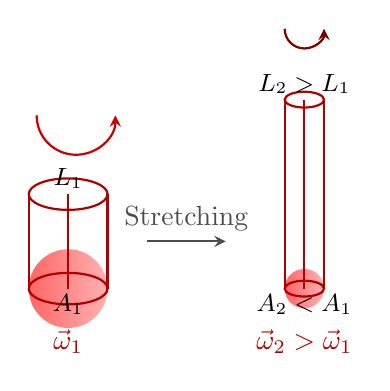
\begin{tikzpicture}[scale=1.0, x={(1cm,0cm)}, y={(0cm,1cm)}, z={(0.3cm,0.2cm)}, >=stealth]
            % Left: initial vortex tube (short & wide)
            \shade[left color=red!60, right color=red!30] (0,0,0) circle (0.5);
            \draw[thick, red!70!black] (0,0,0) ellipse (0.5 and 0.2);
            \draw[thick, red!70!black] (0,0,0) -- (0,1.2,0);
            \draw[thick, red!70!black] (0.5,0,0) -- (0.5,1.2,0);
            \draw[thick, red!70!black] (-0.5,0,0) -- (-0.5,1.2,0);
            \draw[thick, red!70!black] (0,1.2,0) ellipse (0.5 and 0.2);

            \node at (0,-0.2,0) {\small $A_1$};
            \node at (0,1.4,0) {\small $L_1$};
            \node[red!70!black, below] at (0,-0.4) {$\vec{\omega}_1$};

            % Arrow for transformation
            \draw[->, thick, gray!60!black] (1,0.6,0) -- (2,0.6,0) node[midway, above] {Stretching};

             % Front half of the arrow (visible)
            \draw[->, thick, red!80!black]
              (-0.4, 2.2) arc[start angle=180, end angle=360, radius=0.5];

            % Back half (dashed or transparent)
            \draw[->, thick, red!50!black]
              (2.75, 3.3) arc[start angle=180, end angle=360, radius=0.25];

            % Right: stretched vortex tube (tall & thin)
            \shade[left color=red!60, right color=red!30] (3,0,0) circle (0.25);
            \draw[thick, red!70!black] (3,0,0) ellipse (0.25 and 0.1);
            \draw[thick, red!70!black] (3,0,0) -- (3,2.4,0);
            \draw[thick, red!70!black] (3.25,0,0) -- (3.25,2.4,0);
            \draw[thick, red!70!black] (2.75,0,0) -- (2.75,2.4,0);
            \draw[thick, red!70!black] (3,2.4,0) ellipse (0.25 and 0.1);

            \node at (3,-0.2,0) {\small $A_2 < A_1$};
            \node at (3,2.6,0) {\small $L_2 > L_1$};
            \node[red!70!black, below] at (3,-0.4,0) {$\vec{\omega}_2 > \vec{\omega}_1$};
        \end{tikzpicture}
        \caption{Cylindrical representation of vortex stretching.}
        \label{fig:cylinder_vortex_stretching}
    \end{subfigure}%
    \hfill
    \begin{subfigure}[t]{0.48\textwidth}
        \centering
        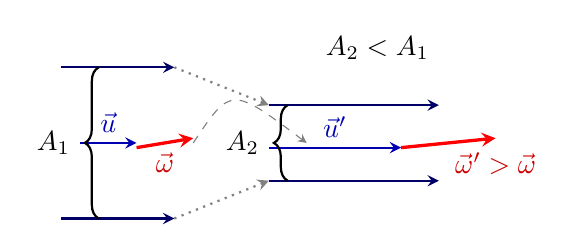
\begin{tikzpicture}[scale=1.2, >=stealth]
            % Left: wide streamlines (converging)
            \draw[->, thick, blue!40!black] (-2,-0.8) -- (-0.8,-0.8);
            \draw[->, thick, blue!40!black] (-2, 0.8) -- (-0.8,  0.8);

            % Transition zone (compression)
            \draw[->, thick, dotted, gray] (-0.8,-0.8) -- (0.2,-0.4);
            \draw[->, thick, dotted, gray] (-0.8, 0.8) -- (0.2, 0.4);

            % Right: narrow streamlines (parallel)
            \draw[->, thick, blue!40!black] (0.2,-0.4) -- (2,-0.4);
            \draw[->, thick, blue!40!black] (0.2, 0.4) -- (2, 0.4);

            % Original vortex filament (shorter)
            \draw[very thick, red, ->] (-1.2,-0.05) -- (-0.6,0.05);
            \node[red!80!black, below] at (-0.9,0) {$\vec{\omega}$};

            % Stretched vortex filament (longer)
            \draw[very thick, red, ->] (1.6,-0.05) -- (2.6,0.05);
            \node[red!80!black, below] at (2.6,0) {$\vec{\omega}' > \vec{\omega}$};

            % Flow velocity vectors
            \draw[->, thick, blue!70!black] (-1.8,0.0) -- (-1.2,0.0) node[midway, above] {$\vec{u}$};
            \draw[->, thick, blue!70!black] (0.2,-0.05) -- (1.6,-0.05) node[midway, above] {$\vec{u}'$};

            % Curved arc to indicate transformation
            \draw[->, dashed, gray] (-0.6,0) .. controls (-0.2,0.6) .. (0.6,0);

            % Area brackets
            \draw[decorate,decoration={brace, amplitude=5pt}, thick] (-1.6,-0.8) -- (-1.6,0.8);
            \node[left] at (-1.8,0) {$A_1$};

            \node[left] at (0.2,0) {$A_2$};
            \draw[decorate,decoration={brace, amplitude=5pt}, thick] (0.4,-0.4) -- (0.4,0.4);
            \node[left] at (2.0,1) {$A_2 < A_1$};
        \end{tikzpicture}
        \caption{Streamline-based view of vortex filament stretching.}
        \label{fig:vortex_stretching_improved}
    \end{subfigure}

    \caption{Two perspectives on vortex stretching in incompressible flow: (a) cylindrical vortex tube conservation, (b) streamline deformation and induced vorticity growth.}
    \label{fig:vortex_stretching_combined}
\end{figure}


In incompressible, inviscid flow, the evolution of vorticity \( \vec{\omega} \equiv \nabla \times \vec{u} \) is governed by deformation of vortex lines due to velocity gradients. Starting from the inviscid Navier--Stokes equation:
\[
\frac{\partial \vec{u}}{\partial t} + (\vec{u} \cdot \nabla)\vec{u} = -\frac{1}{\rho} \nabla p,
\]
we take the curl of both sides:
\[
\frac{\partial}{\partial t} (\nabla \times \vec{u}) + \nabla \times \left[ (\vec{u} \cdot \nabla)\vec{u} \right] = 0.
\]
Recognizing the vorticity \( \vec{\omega} = \nabla \times \vec{u} \), and applying the identity:
\[
\nabla \times \left[ (\vec{u} \cdot \nabla)\vec{u} \right] = (\vec{\omega} \cdot \nabla)\vec{u} - (\vec{u} \cdot \nabla)\vec{\omega},
\]
we derive the vorticity transport equation:
\[
\frac{\partial \vec{\omega}}{\partial t} + (\vec{u} \cdot \nabla)\vec{\omega} = (\vec{\omega} \cdot \nabla)\vec{u},
\]
which simplifies using the material derivative:
\begin{equation}
\boxed{ \frac{D \vec{\omega}}{D t} = (\vec{\omega} \cdot \nabla)\vec{u} }
\end{equation}

\textbf{Interpretation:} The right-hand side represents the \emph{vortex stretching term}. It governs the increase in vorticity magnitude when a vortex filament is stretched by the flow. When a velocity gradient aligns with the direction of vorticity, angular momentum conservation causes the rotation rate to intensify.

\medskip

\textit{Analogy:} Pulling on a spinning elastic band makes it spin faster. Vortex filaments behave similarly under æther flow deformation.

\begin{flushright}
    \textbf{Reference:} G. K. Batchelor, \textit{An Introduction to Fluid Dynamics}, Cambridge University Press, 2000.
\end{flushright}
\end{tcolorbox}


    \subsubsection{Derivation of Vorticity-Based Fluid Equations}
    The equation for u:
    \begin{equation}
        \frac{d u}{d t}+u \frac{d u}{d \boldsymbol{x}}+v \frac{d u}{d y}-\zeta_{\text {atom}} v=-g \frac{d \eta}{d \boldsymbol{x}}+\mathcal{R}_x\label{eq:momentum_u}
    \end{equation}

    the equation for v:
    \begin{equation}
        \frac{d v}{d t}+u \frac{d v}{d x}+v \frac{d v}{d y}+\zeta_{\text {atom }} u=-g \frac{d \eta}{d y}+\mathcal{R}_v\label{eq:momentum_v}
    \end{equation}
    are a form of the \textbf{momentum equation} for the velocity components $u$ and $v$, incorporating vorticity, gravity effects, and external
    forcing
    terms.

    \begin{itemize}
        \item \textbf{Material Derivative} $\frac{d u}{d t}$: Represents the total derivative (substantial derivative) following a fluid parcel.
        \item \textbf{Convective Terms} $u \frac{d u}{dx} + v \frac{d u}{dy}$: Describe how velocity gradients impact acceleration.
        \item \textbf{Vorticity Term} $-\zeta_\text{atom} u$: Arises from the influence of vorticity on velocity evolution.
        \item \textbf{Gravity-Induced Term} $-g \frac{d \eta}{d x}$: Represents pressure gradient due to gravity.
        \item \textbf{External Forcing Term} $\mathcal{R}_x$: Represents additional external forces such as resistive or turbulent effects.
    \end{itemize}

    This equation is derived from the \textbf{Navier-Stokes Equations} under the assumption of an inviscid, incompressible fluid with rotational
    effects.
    We will from now on now use $\zeta_\text{atom} \rightarrow \zeta_\text{a} $

    \subsubsection*{Differentiation with Respect to $y$}
    Differentiating the equation ~\ref{eq:momentum_u} with respect to $y$:
    \begin{equation*}
        \frac{d}{dy} \left( \frac{d u}{d t} + u \frac{d u}{d x} + v \frac{d u}{d y} - \zeta_\text{a} v \right) = \frac{d}{dy} \left( - g
                                                                                                                                   \frac{d \eta}{d x} + \mathcal{R}_x \right)
    \end{equation*}
    Expanding this:
    \begin{align}
        \frac{d^2 u}{d t d y}+\frac{d u}{d y} \frac{d u}{d x}+u \frac{d^2 u}{d x d y}+\frac{d v}{d y} \frac{d u}{d y}+v \frac{d^2 u}{d y^2}-\zeta_a \frac{d v}{d y}-\beta v=-g \frac{d^2 \eta}{d x d y}+\frac{d \mathcal{R}_x}{d y}
    \end{align}

    Similarly, differentiating the equation~\ref{eq:momentum_v} for $v$ with respect to $x$:
    \begin{equation*}
        \frac{d}{dx} \left( \frac{d v}{d t}+u \frac{d v}{d x}+v \frac{d v}{d y}+\zeta_{\text {a}} u \right) =  \frac{d}{dx} \left( -g
                                                                                                                                 \frac{d \eta}{d y}+\mathcal{R}_v \right)
        \label{eq:diff_v_to_x}
    \end{equation*}
    Differentiating with respect to $x$:
    \begin{align}
        \frac{d^2 v}{d t d x}+\frac{d u}{d x} \frac{d v}{d x}+u \frac{d^2 v}{d x^2}+\frac{d v}{d x} \frac{d v}{d y}+v \frac{d^2 v}{d x d y}+\zeta_a \frac{d u}{d x}=-g \frac{d^2 \eta}{d x d y}+\frac{d \mathcal{R}_w}{d x}
    \end{align}

    \subsubsection*{Combination of the Two Equations}
    By adding both derived equations, we get:
    \begin{eqbox}
        \begin{equation}
        \frac{\delta \zeta}{\delta t}+\zeta \frac{d u}{d x}+u \frac{\delta \zeta}{\delta x}+\zeta \frac{d v}{d y}+v \frac{\delta \zeta}{\delta y}+\zeta_a\left(\frac{d u}{d x}+\frac{d v}{d y}\right)+\beta v=\frac{d \mathcal{R}_v}{d x}-\frac{d \mathcal{R}_x}{d y}
        \end{equation}
    \end{eqbox}
    which is a vorticity-based formulation of the original momentum equations.

    \subsubsection*{Representation of Forcing Terms}
    In the presence of external forcing and turbulence:
    \begin{align}
        \mathcal{R}_x &= \frac{1}{\rho}(\tau_x^w - \tau_x^v)
    \end{align}
    \begin{align}
        \mathcal{R}_y &= \frac{1}{\rho}(\tau_y^w - \tau_y^b)
    \end{align}
    where $\tau_x^w, \tau_x^v, \tau_y^w, \tau_y^b$ represent the stress terms.

    \subsubsection{Final Vorticity Equation}
    \begin{eqbox}
        \begin{equation}
        \frac{D \zeta}{d t}-\frac{\zeta_r+\zeta_a}{h} \frac{D h}{d t}+\frac{D \zeta_a}{d t}=\frac{d R_u}{d x}-\frac{d R_x}{d y}
        \end{equation}
    \end{eqbox}
    This equation models higher-order vortex interactions, crucial for understanding turbulence, energy dissipation, and wave-vortex interactions.

    \subsubsection*{Conclusion}
    The derivation follows classical fluid dynamics principles and extends into turbulence modeling. These equations are significant in vortex dynamics, superfluid behavior, and atmospheric circulations. They also appear in various studies on vortex ring dynamics.

    \subsection{Governing Vorticity Transport Equation}
    The fundamental vorticity equation is:
    \begin{equation}
        \frac{\partial \zeta}{\partial t} + u \frac{\partial \zeta}{\partial x} + v \frac{\partial \zeta}{\partial y} + \left( \zeta_r + \zeta_a \right) \left( \frac{\partial u}{\partial x} + \frac{\partial v}{\partial y} \right) + \beta v = \frac{\partial \mathcal{R}_v}{\partial x} - \frac{\partial \mathcal{R}_x}{\partial y}
    \end{equation}
    where:
    \begin{itemize}
        \item $\zeta$ is the \textbf{relative vorticity}.
        \item $\zeta_r$ and $\zeta_a$ represent \textbf{relative and absolute vorticity contributions}.
        \item $\beta v$ is the \textbf{beta-effect}, modeling the variation of planetary vorticity with latitude.
        \item $\mathcal{R}_x, \mathcal{R}_y$ are external forcing terms, such as frictional forces or turbulence-induced vorticity changes.
    \end{itemize}

    \subsection{Vorticity in Height-Dependent Flow}
    \begin{equation*}
        \frac{D \zeta}{d t} - \frac{ \zeta_r + \zeta_a }{h}  \frac{D h}{d t} + \frac{D \zeta_a}{d t}  = \frac{\partial \mathcal{R}_y}{\partial x} - \frac{\partial \mathcal{R}_x}{\partial y}
    \end{equation*}
    This ensures vorticity conservation even in \textbf{variable-height flows}, such as oceanic or atmospheric circulations.

    \subsubsection*{Barotropic Vorticity Equation and Potential Vorticity}
    \begin{equation}
        D\left(\frac{\zeta_r+\zeta_a}{h}\right)=\frac{1}{h}\left(\frac{d R_y}{d x}-\frac{d R_x}{d y}\right)
    \end{equation}
    The \textbf{Potential Vorticity (PV)} is conserved:
    \begin{equation}
        \Pi = \frac{\zeta_a+\zeta_r}{h}
    \end{equation}
    This is crucial for \textbf{understanding Rossby waves, planetary circulation, and stratified fluid dynamics}.

    \subsubsection*{Relationship to Streamfunction}
    \begin{equation}
        \boxed{\zeta = \nabla^2 \psi}
    \end{equation}
    The vorticity field is linked to the \textbf{streamfunction} through the Laplacian operator.

    \subsubsection{Absolute Vorticity and Coriolis Terms}
    \begin{align}
        f &= 2 \omega, \quad \zeta=-\alpha \\
        \zeta_\text{atom} &= 2 \omega \sin (\theta) \\
        \zeta_\text{Absolute} &= \zeta_\text{atom }+\zeta_\text{relative}
    \end{align}
    Absolute vorticity is the sum of relative vorticity and the Coriolis parameter.

    \subsubsection{Conservation of Vorticity}
    \begin{equation*}
        \frac{D \zeta}{D t}=0=\frac{\partial \zeta}{\partial t}+u \cdot \nabla \zeta
    \end{equation*}
    In an inviscid flow, vorticity is conserved along streamlines.

    \begin{equation}
        \frac{\partial \zeta}{\partial t} + u \cdot \nabla(\zeta + f)=0
    \end{equation}

    Where when the Coriolis term $\zeta_a$ is constant, and the equation simplifies to:

    \begin{eqbox}
    \begin{equation}
        \frac{\partial \zeta}{\partial t}+J(\psi, \nabla^2 \psi)=0
    \end{equation}
    \end{eqbox}

    This is used in \textbf{geophysical fluid dynamics}, where $J(\psi, \nabla^2 \psi)$ is the Jacobian term representing nonlinear advection in
    two-dimensional flows.

    \subsubsection*{Conclusion}
    These equations describe the \textbf{evolution of vorticity in a rotating fluid with height variations and external forcing effects}. They are foundational for:
    \begin{itemize}
        \item Geophysical fluid dynamics (GFD).
        \item Turbulence modeling.
        \item Vortex dynamics in atmospheric and oceanic flows.
    \end{itemize}
    This framework allows for \textbf{wave-vortex interactions}, barotropic/baroclinic instabilities, and the development of \textbf{cyclonic systems}.


        \section{Entropic Gravity from Vortex Swirl Thermodynamics}

    We adopt Verlinde’s entropic force framework \cite{verlinde2010emergent}, where gravity emerges not as a fundamental force but from changes in information entropy across spatial displacements. In the Vortex Æther Model (VAM), this is reinterpreted through swirl-induced pressure gradients in the æther.

    Verlinde's force law:
    \[
        F = T \frac{\Delta S}{\Delta x}
    \]
    is realized in VAM via pressure gradients resulting from varying swirl intensity. The entropy gradient is modeled using the Unruh relation:
    \[
        \Delta S = 2\pi k_B \frac{mc}{\hbar} \Delta x
    \]
    This maps to vortex energy stored in tangential motion.

    We define a local swirl-based effective temperature as:
    \[
        T_\text{eff} = \frac{1}{2k_B} \rho_{\text{\ae}} \Omega^2 r^2
    \]
    yielding a force:
    \[
        F = -\nabla P = -\nabla \left( \frac{1}{2} \rho_{\text{\ae}} \Omega^2 r^2 \right)
    \]
    This reproduces the entropic force law as a physical manifestation of pressure gradients within structured vortex flow. Here, mass corresponds to integrated swirl energy, and displacement alters entropy via vortex configuration change.

    \begin{table}[H]
        \centering
        \caption{Conceptual Correspondence: Verlinde's Entropic Gravity and VAM}
        \footnotesize
        \begin{tabular}{|l|l|}
            \hline
            \textbf{Verlinde Concept} & \textbf{VAM Interpretation} \\
            \hline
            Entropy gradient & Swirl-induced pressure drop \\
            Holographic screen & Vortex boundary with helicity content \\
            Equipartition energy & Core quantized swirl energy \\
            Unruh effect & Swirl-induced effective temperature \\
            Inertial mass from $\Delta S$ & Swirl resistance to displacement \\
            Bits on screen & Quantized circulation or helicity units \\
            \hline
        \end{tabular}
    \end{table}



    \section{Temporal Coupling Between Rotational and Translational Æther Dynamics}

    \textbf{Rigid Rotor Dynamics:} Each vortex knot is modeled as a rigidly rotating entity, maintaining a stable angular velocity throughout its core under Vortex Proper Time \( T_v \). These cores are assumed to deform minimally, preserving their rotation under ideal conditions.

    \textbf{Vorticity as a Vector Field:} The vorticity vector for each knot is aligned with the Z-axis:
    \begin{equation*}
        \vec{\omega} = \omega \hat{z},
    \end{equation*}
    which simplifies analysis and reflects cylindrical symmetry in the ætheric vortex tube.

    \textbf{Kinematic Parameters:}
    \begin{itemize}
        \item \textbf{Spatial positions:} Knots are located at \( z_1 \) and \( z_2 \) along the Z-axis.
        \item \textbf{Axial velocities (Chronos-Time):}
        \begin{equation*}
            v_1 = \frac{dz_1}{d\tau_1}, \quad v_2 = \frac{dz_2}{d\tau_2}.
        \end{equation*}
        \item \textbf{Relative velocity:}
        \begin{equation*}
            v_\text{rel} = \frac{d(z_2 - z_1)}{d\mathcal{N}},
        \end{equation*}
        which measures spatial separation rate in absolute Aithēr-Time \( \mathcal{N} \).
    \end{itemize}

    \textbf{Vortex Tube Structure:} A connecting vortex tube with uniform vorticity transmits angular momentum along \( z \), coupling the two knots dynamically.

    \textbf{Æther Properties:} The surrounding æther is modeled as incompressible and inviscid, enabling conservative transmission of vorticity and swirl pressure without dissipative losses.

    \subsection{Derivation of Relative Vorticity}

    \textbf{Vorticity Difference:}
    \begin{equation*}
        \Delta \omega = \omega_2 - \omega_1,
    \end{equation*}
    where each angular velocity evolves along its respective vortex in proper time:
    \begin{equation*}
        \omega_1 = \frac{d\theta_1}{dT_{v1}}, \quad \omega_2 = \frac{d\theta_2}{dT_{v2}}.
    \end{equation*}

    \textbf{Relative Angular Displacement:}
    \begin{equation*}
        \Delta \omega = \omega_\text{rel} = \frac{d(\theta_2 - \theta_1)}{d\mathcal{N}}.
    \end{equation*}
    This projects the time evolution of rotational disparity into the global causal frame \( \mathcal{N} \), ensuring frame-independent vortex coupling.

    \subsection*{Translational–Rotational Coupling}

    \textbf{Vorticity–Velocity Mapping:}
    \begin{equation*}
        \omega_\text{rel}(d\mathcal{N}) = C \frac{v_2 - v_1}{|z_2 - z_1|},
    \end{equation*}
    where \( v_i = \frac{dz_i}{d\tau_i} \) are measured in local Chronos-Time \( \tau_i \). The constant \( C \) encodes the vortex tube’s
inertial and elastic response properties. This coupling relation does not appear explicitly in classical hydrodynamics, but bears conceptual similarity to axial–rotational energy exchange mechanisms in Rossby-type wave–vortex systems~\cite{rossby1939} and classical vortex tube theory~\cite{lamb1932, batchelor2000}.


\subsection{Interpretation in Temporal Ontology}

    \begin{itemize}
        \item \textbf{Temporal Layering:}
        - Vortex rotations evolve in \( T_v \),
        - Translational flow in \( \tau \),
        - Their interaction is projected onto \( \mathcal{N} \), providing a unified causal metric.

        \item \textbf{Spatial Scaling:} The term \( |z_2 - z_1| \) reflects inverse distance scaling typical of fluid vortex interactions.

        \item \textbf{Energetic Feedback:} Increases in \( v_\text{rel} \) (Chronos) drive higher \( \omega_\text{rel} \) (Swirl Clock acceleration), redistributing kinetic energy within the tube.
    \end{itemize}

    \subsection*{Energy Transfer Implications}

    This time-mode-aware formulation supports a VAM-based energy transport mechanism where vortex-to-vortex coupling transmits angular information along \( \mathcal{N} \), modulating Swirl Clocks \( S(t) \) and altering time dilation rates in surrounding æther regions.

    \subsection*{Conclusion}

    This refined derivation aligns the rotational-translational dynamics of vortex knots with the layered time framework of the Vortex Æther Model. By mapping proper times \( T_v, \tau \), and the global causal time \( \mathcal{N} \) into a unified structure, we obtain a temporally coherent view of vortex interactions. Future research may explore non-linearities in \( C \), and energy bifurcations (Kairos moments \( \kappa \)) as topological instabilities in the vortex chain.


        \section{Kairos Moments and Topological Transitions in VAM}

    \subsection*{Overview}
    In the Vortex \AE{}ther Model (VAM), time is structured into distinct modes:
    \begin{itemize}
        \item \textbf{Aith\={e}r-Time} (\( \mathcal{N} \)): universal causal background
        \item \textbf{Chronos-Time} (\( \tau \)): proper time along macroscopic trajectories
        \item \textbf{Swirl Clock} (\( S(t) \)): local clock rate modulated by vorticity energy
        \item \textbf{Vortex Proper Time} (\( T_v \)): time along rotating core structures
        \item \textbf{Kairos Moment} (\( \kappa \)): irreversible topological or energetic bifurcation
    \end{itemize}
    Among these, \( \kappa \) marks critical transition points where smooth time evolution in \( \mathcal{N} \) or \( \tau \) cannot be maintained.

    \subsection{Definition of a Kairos Moment}
    A \textit{Kairos Moment} \( \kappa \) is defined as a non-analytic point in the evolution of the vortex æther field, typically accompanied by a discontinuity in the temporal or topological structure:
    \begin{equation}
        \lim_{\epsilon \to 0} \left( \frac{d\vec{\omega}}{dt} \right)_{t = \kappa - \epsilon}
        \neq
        \left( \frac{d\vec{\omega}}{dt} \right)_{t = \kappa + \epsilon}.
    \end{equation}

    Such moments correspond to irreversible events like:
    \begin{itemize}
        \item vortex reconnection,
        \item knot topological transitions (\( \Delta Lk \in \mathbb{Z} \)),
        \item swirl energy overloads,
        \item swirl clock rate rupture.
    \end{itemize}


    \begin{figure}[h]
        \centering
        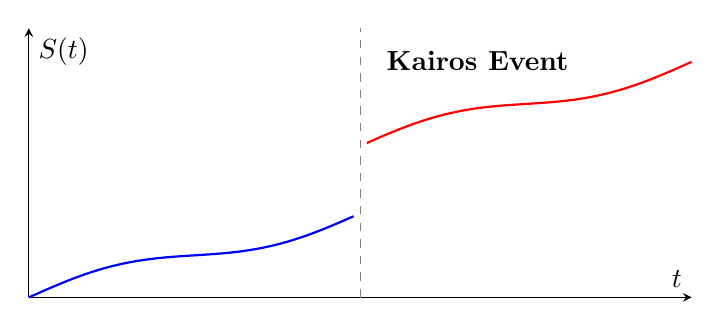
\begin{tikzpicture}

            \begin{axis}[
            axis lines=middle,
            xlabel={$t$},
            ylabel={$S(t)$},
            xtick=\empty,
            ytick=\empty,
            xmin=0, xmax=10,
            ymin=0, ymax=8,
            width=10cm,
            height=5cm,
            samples=100,
            domain=0:10,
            smooth,
            clip=false
            ]

% Swirl clock function before jump
            \addplot[thick, blue, domain=0:4.9] {0.5*x + 0.3*sin(deg(2*pi*x/5))};
% After jump
            \addplot[thick, red, domain=5.1:10] {0.5*x + 0.3*sin(deg(2*pi*x/5)) + 2};

% Kairos event line
            \addplot[dashed, gray] coordinates {(5,0) (5,8)};

            \end{axis}

% Kairos label above the dashed line
            \node at (5.7,3.0) {\textbf{Kairos Event}};

        \end{tikzpicture}
        \caption{Swirl clock bifurcation at $t = t_c$: a topological reconnection causes a discrete phase shift in $S(t)$.}
    \end{figure}


    \subsection{Trigger Conditions for Kairos Transitions}
\begin{eqbox}
    \begin{table}[H]
        \centering
        \footnotesize
        \renewcommand{\arraystretch}{1.4}
        \begin{tabular}{|c|l|l|}
            \hline
            \textbf{Type} & \textbf{Trigger Condition} & \textbf{Physical Interpretation} \\
            \hline
            \textbf{1. Vorticity Gradient Singularity} &
            $|\nabla \vec{\omega}| \geq \dfrac{C_e}{r_c^2}$ &
            Core rupture or instability onset \\
            \textbf{2. Helicity Discontinuity} &
            $\Delta H \neq 0$, $\Delta Lk \in \mathbb{Z}$ &
            Knottedness transition \\
            \textbf{3. Energy Threshold Exceeded} &
            $U_{\text{swirl}} > U_{\text{max}} = \frac{1}{2} \rho_{\text{\ae}} C_e^2$ &
            Collapse from over-rotation \\
            \textbf{4. Vortex Collision} &
            $\vec{\omega}_1 \cdot \vec{\omega}_2 < 0$, at $|\vec{r}_1 - \vec{r}_2| < \delta r_c$ &
            Reconnection or annihilation \\
            \textbf{5. Swirl Clock Discontinuity} &
            $\left.\frac{dS}{dt}\right|_{t = \kappa^-} \neq \left.\frac{dS}{dt}\right|_{t = \kappa^+}$ &
            Local time rupture in vortex cores \\
            & & \\
            \hline
        \end{tabular}
        \caption{Trigger conditions for Kairos transitions in the vortex æther field.}\label{tab:table}
    \end{table}
\end{eqbox}

    \subsection{Energetic Criterion from Swirl Potential}
    Kairos events are energetically triggered when local swirl energy exceeds the maximum sustainable value in the æther medium:
    \begin{equation}
        U_{\text{swirl}} = \frac{1}{2} \rho_{\text{\ae}} |\vec{\omega}|^2,
        \quad
        U_{\text{max}} = \frac{1}{2} \rho_{\text{\ae}} C_e^2.
    \end{equation}
    Hence, the condition:
    \[
        U_{\text{swirl}} > U_{\text{max}}
    \]
    triggers structural realignment, swirl rupture, or reconnection.

    \subsection{Helicity and Knot Transitions}
    The total helicity \( H \) of a vortex system is given by:
    \begin{equation}
        H = \int \vec{v} \cdot \vec{\omega} \, dV,
    \end{equation}
    which is conserved under smooth evolution. However, when:
    \[
        \Delta H = H_{\text{after}} - H_{\text{before}} \neq 0,
    \]
    a topological transformation has occurred, such as knot reconnection or linking number jump (\( \Delta Lk \in \mathbb{Z} \)) — a definitive marker of \( \kappa \).

    \subsection{Temporal Discontinuity in Swirl Clocks}
    Swirl clocks \( S(t) \) track local time using vorticity-based rates. A Kairos moment induces a discontinuity in the swirl time derivative:
    \begin{equation}
        \lim_{\epsilon \to 0} \left[ \frac{dS}{dt}(t = \kappa - \epsilon) \right]
        \neq
        \left[ \frac{dS}{dt}(t = \kappa + \epsilon) \right].
    \end{equation}
    This represents an irreversible reconfiguration of the internal clock rate, isolating vortex epochs before and after \( \kappa \).

    \subsection{Interpretation Across Time Modes}

    \begin{table}[H]
        \centering
        \renewcommand{\arraystretch}{1.3}
        \begin{tabular}{|c|c|p{9cm}|}
            \hline
            \textbf{Time Mode} & \textbf{Symbol} & \textbf{Effect at Kairos Moment} \\
            \hline
            Aithēr-Time & \( \mathcal{N} \) & Globally continuous, but re-indexed at \(\kappa\) \\
            Chronos-Time & \( \tau \) & Broken derivative continuity (\( d\tau/dt \) jump) \\
            Swirl Clock & \( S(t) \) & Discontinuous rate: \( \Delta \left(\frac{dS}{dt}\right) \neq 0 \) \\
            Vortex Proper Time & \( T_v \) & Reset or bifurcation of local vortex clock phase \\
            Kairos Marker & \( \kappa \) & Singular time point; cannot be evolved through \\
            \hline
        \end{tabular}
        \caption{Temporal ontology response to a Kairos transition.}
    \end{table}


    \subsection{Experimental Analogy}
    An accessible analogy to Kairos transitions exists in superfluid helium (\(^4\)He), where vortex reconnections are captured by tracer
    particles and Kelvin waves~\cite{bewley2006} These observations reveal the discontinuous evolution of topological structures, paralleling the role of \( \kappa \) in VAM.

    \subsection*{Conclusion}
    Kairos Moments \( \kappa \) encode the breakdown of smooth time evolution in the Vortex Æther Model. They delineate epochs of distinct
    topological and energetic configurations, demarcate irreversible transitions, and formalize events beyond the classical conservation paradigm. These singularities lie at the intersection of topology, dynamics, and temporality — and serve as central markers in vortex chronology. While the concept of Kairos Moments is novel to the Vortex Æther Model, it draws inspiration from quantized vortex reconnections observed in superfluid helium~\cite{bewley2006}, helicity transitions in classical fluid dynamics~\cite{moffatt1969}, and non-analytic behavior in phase transitions~\cite{landau1959}.


        \section{Vorticity and Time Dilation in the Vortex Æther Model (VAM)}


In VAM, local time flow is governed not by spacetime curvature, but by the relative velocity and vorticity of the æther swirl. We define a local swirl-based clock \( S(t) \) whose proper time dilation arises from the vorticity field:

\[
    \frac{d\tau}{dt} = \sqrt{1 - \frac{|\vec{v}_{\text{swirl}}|^2}{c^2}} = \sqrt{1 - \frac{|\vec{\omega} \times \vec{r}|^2}{c^2}}
\]

This generalizes the usual gravitational time dilation by reinterpreting gravity as a pressure and swirl gradient. The swirl velocity \( \vec{v}_{\text{swirl}} \) is locally induced by the circulation density \( \vec{\omega} \), giving rise to anisotropic clock rates depending on vortex alignment and intensity.

\subsection{Effective Lagrangian for Swirl Quantization}

To model the quantized nature of the ætheric swirl fields and their backreaction on local time structure, we introduce a prototype Lagrangian density:

\[
    \mathcal{L} = \frac{1}{2} \rho_{\scriptscriptstyle\boldsymbol\!f} \left( \partial_t \vec{\psi} \cdot \partial_t \vec{\psi} - c^2 \nabla \vec{\psi} \cdot \nabla \vec{\psi} \right) - V(\vec{\psi}) - \lambda \, \epsilon^{ijk} \psi_i \partial_j \psi_k
\]

Here, \( \vec{\psi} \) is the swirl potential field, with vorticity \( \vec{\omega} = \nabla \times \vec{\psi} \). The term:

- \( V(\vec{\psi}) = \frac{1}{2} m^2 |\vec{\psi}|^2 + \frac{\beta}{4} |\vec{\psi}|^4 \) introduces self-interactions, allowing vortex condensation.
- \( \epsilon^{ijk} \psi_i \partial_j \psi_k \) This helicity term quantizes the circulation through topological constraints, enforcing minimal helicity quanta.

\subsection{Quantized Time Flow and Helicity Defects}

Swirl quantization implies discrete `jumps` in the swirl clock \( S(t) \), especially at topological reconnection events. These moments correspond to \textbf{Kairos-time bifurcations} and are mathematically modeled as phase slips in the vortex field \( \vec{\psi} \), similar to those in superfluid systems.

At critical vorticity thresholds, the energy density near the vortex core causes:

\[
    \Delta t_{\text{dilated}} = \int \left( 1 - \frac{|\vec{\omega}(r)|^2}{c^2} \right)^{1/2} dr
\]

signifying the temporal effect of finite-size vortex domains on clock synchronization. Thus, time dilation is an emergent, field-induced phenomenon rooted in local swirl configuration.


    \section{Swirl Clocks, Entropy, and the Time Phase Field}

    We interpret the swirl clock \( S(t) = \int \Omega(t') dt' \) not only as a cumulative phase, but as a local entropy memory. Changes in \( S \) correspond to local thermodynamic gradients driving vortex-induced acceleration.

    Following Verlinde’s idea of discrete information bits on holographic screens, VAM substitutes topological quantization:
    \[
        N_{\text{bits}} \longleftrightarrow \sum_i \Gamma_i^2 (T + W)
    \]
    where \( \Gamma_i \) is the circulation quantum of vortex tube \( i \), and \( T \), \( W \) denote twist and writhe. This connects information content to helicity topology, and entropy to swirl entanglement.

    \subsection{Variational Action for the Swirl Phase Field}

    We now propose a dynamical action for the time-phase field \( S(x, t) \), treated as a scalar describing the evolution of local clock structure:

    \[
        \mathcal{A}_S = \int d^4x \left[ \frac{\rho_{\text{\ae}}}{2} (\partial_t S)^2 - V(S) + \alpha \{S, t\} \right]
    \]

    Here:
    - \( V(S) = \frac{1}{2} m^2 S^2 + \frac{\beta}{4} S^4 \) represents potential energy from swirl density variations.
    - The Schwarzian derivative:
    \[
        \{S, t\} = \frac{\dddot{S}}{\dot{S}} - \frac{3}{2} \left( \frac{\ddot{S}}{\dot{S}} \right)^2
    \]
    captures the chaotic geometry of time bifurcations during topological transitions (Kairos events). This term is also relevant in conformal mechanics, JT gravity, and turbulence onset.

    The action \(\mathcal{A}_S\) provides a dynamical basis for swirl clock evolution, where discrete reconnections or helicity jumps induce nonlinear phase dynamics.

    Such discontinuities correspond to physical breakdowns of analytic time—transitions between distinct temporal topologies. The appearance of the Schwarzian is both a signal of symmetry breaking and a geometrical measure of temporal instability.


    \begin{figure}[h]
        \centering
        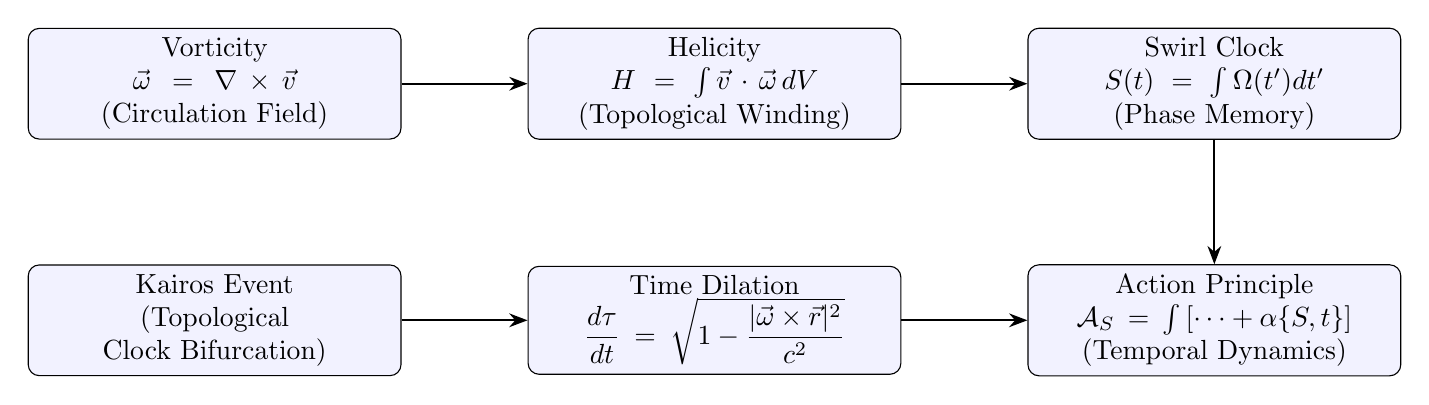
\begin{tikzpicture}[node distance=1.6cm and 1.6cm]

% Top Row
            \node (vorticity) [block] {Vorticity\\$\vec{\omega} = \nabla \times \vec{v}$\\(Circulation Field)};
            \node (helicity) [block, right=of vorticity] {Helicity\\$H = \int \vec{v} \cdot \vec{\omega}\, dV$\\(Topological Winding)};
            \node (swirlclock) [block, right=of helicity] {Swirl Clock\\$S(t) = \int \Omega(t') dt'$\\(Phase Memory)};

% Bottom Row
            \node (timedilation) [block, below=of helicity] {Time Dilation\\$\displaystyle\frac{d\tau}{dt} = \sqrt{1 - \frac{|\vec{\omega} \times \vec{r}|^2}{c^2}}$};
            \node (action) [block, right=of timedilation] {Action Principle\\$\mathcal{A}_S = \int \left[ \cdots + \alpha\{S,t\} \right]$\\(Temporal Dynamics)};
            \node (kairos) [block, left=of timedilation] {Kairos Event\\(Topological Clock Bifurcation)};

% Horizontal Arrows
            \draw [arrow] (vorticity) -- (helicity);
            \draw [arrow] (helicity) -- (swirlclock);

% Down Arrows
            \draw [arrow] (swirlclock) -- (action);

% Bottom Row Arrows
            \draw [arrow] (timedilation) -- (action);
            \draw [arrow] (kairos) -- (timedilation);

        \end{tikzpicture}
        \caption{Condensed conceptual flow: from vorticity to temporal bifurcation in the VAM framework}
    \end{figure}

    \section{Conclusion, Discussion, and Outlook}

    In this work, we have advanced a novel fluid-dynamic formulation of gravity and time, grounded in the dynamics of a structured, incompressible æther. By reinterpreting gravitational attraction as the result of pressure gradients induced by quantized swirl, and local time as a function of motion through vorticity fields, we offer an alternative to metric-based curvature models. The Vortex Æther Model (VAM) unifies inertial and gravitational phenomena through relative circulation and introduces the concept of \emph{swirl clocks} as the governing principle of local temporal flow.

    Our analysis bridges classical vorticity dynamics with relativistic time dilation, extending into topological fluid mechanics via helicity conservation and vortex reconnection. The introduction of \emph{Kairos events}—singular bifurcations in the swirl topology—marks a departure from purely analytic treatments of time and allows for discrete, physical manifestations of non-linearity in clock evolution. Moreover, the formulation of an effective swirl field Lagrangian opens a path toward quantized models of ætheric structure, positioning the model alongside contemporary field theories and condensed matter analogs.

    The implications are both foundational and testable. On one hand, VAM provides a conceptual resolution to long-standing tensions between Machian inertia, entropic gravity, and relativistic time. On the other, it suggests experimental avenues involving Sagnac interferometry, superfluid analogs, and clock synchronization anomalies in strong-vorticity regions. Notably, the reinterpretation of light speed as a swirl-limited propagation velocity offers fresh insight into variable-\( c \) cosmologies and Rømer-type measurements.

    Looking forward, several critical directions emerge:

    \begin{itemize}
        \item \textbf{Field Quantization:} Developing a full quantized field theory for the swirl potential \( \vec{\psi} \), including vortex interactions and boundary effects.
        \item \textbf{Gravitational Collapse:} Refining the VAM analog of Schwarzschild collapse in terms of swirl energy depletion and pressure null surfaces.
        \item \textbf{Temporal Topology:} Formalizing Kairos events via Morse theory or topological transitions in a fiber bundle structure of time.
        \item \textbf{Experimental Probes:} Designing interferometric or quantum optical tests to detect swirl-induced time gradients or helicity-induced phase shifts.
        \item \textbf{Cosmological Modeling:} Applying the VAM framework to large-scale structure, horizon formation, and the time evolution of constants such as \( G \), \( \hbar \), and \( c \).
    \end{itemize}

    By extending the language of fluid mechanics into the temporal and gravitational domains, this model proposes not just a reinterpretation of known physics, but a new ontology of time and motion. In doing so, it invites both rigorous mathematical development and innovative experimental testing at the intersection of topology, field theory, and cosmology.


\begin{thebibliography}{99}

\bibitem{helmholtz1858integralsvortex}
Hermann von Helmholtz,
\newblock Über Integrale der hydrodynamischen Gleichungen, welche den Wirbelbewegungen entsprechen.
\textit{Journal für die reine und angewandte Mathematik (Crelle's Journal)} \textbf{55}, 25--55 (1858).
\newblock DOI: \href{https://doi.org/10.1515/crll.1858.55.25}{10.1515/crll.1858.55.25}.
\newblock English translation: ``On the integrals of the hydrodynamic equations which express vortex motion''.


\bibitem{maxwell1861pressure}
James Clerk Maxwell,
\newblock On Physical Lines of Force.
\textit{Philosophical Magazine} \textbf{21} (139--145), 161--175, 281--291, 338--348, 469--512 (1861).
\newblock \url{https://en.wikisource.org/wiki/On_Physical_Lines_of_Force}.
\newblock Four-part series.


\bibitem{lamb1932}
Horace Lamb,
\newblock Hydrodynamics.
\newblock Cambridge University Press, 1932.


\bibitem{rossby1939}
Carl-Gustaf Rossby,
\newblock Relations between Variations in the Intensity of the Zonal Circulation of the Atmosphere and the Displacements of the Semi-Permanent Centers of Action.
\textit{Journal of Marine Research} \textbf{2} (1), 38--55 (1939).
\newblock Classic formulation of potential vorticity and planetary wave dynamics.


\bibitem{pedlosky1987}
Joseph Pedlosky,
\newblock Geophysical Fluid Dynamics.
\newblock Springer, 1987.
\newblock DOI: \href{https://doi.org/10.1007/978-1-4612-4650-3}{10.1007/978-1-4612-4650-3}.


\bibitem{verlinde2010emergent}
Verlinde, Erik P.,
\newblock On the Origin of Gravity and the Laws of Newton.
\textit{Journal of High Energy Physics} \textbf{2011} (4), 29 (2011).
\newblock DOI: \href{https://doi.org/10.1007/JHEP04(2011)029}{10.1007/JHEP04(2011)029}.


\bibitem{batchelor2000}
G. K. Batchelor,
\newblock An Introduction to Fluid Dynamics.
\newblock Cambridge University Press, 2000.


\bibitem{bewley2006}
Bewley, G. P. and Paoletti, M. S. and Sreenivasan, K. R. and Lathrop, D. P.,
\newblock Superfluid helium: Visualization of quantized vortices.
\textit{Nature} \textbf{441} (7093), 588 (2006).
\newblock DOI: \href{https://doi.org/10.1038/441588a}{10.1038/441588a}.


\bibitem{moffatt1969}
H. K. Moffatt,
\newblock The degree of knottedness of tangled vortex lines.
\textit{Journal of Fluid Mechanics} \textbf{35} (1), 117--129 (1969).
\newblock DOI: \href{https://doi.org/10.1017/S0022112069000991}{10.1017/S0022112069000991}.


\bibitem{landau1959}
L. D. Landau and E. M. Lifshitz,
\newblock Fluid Mechanics.
\newblock Pergamon, 1959.


\end{thebibliography}


\end{document}